\documentclass{article}\usepackage[]{graphicx}\usepackage[]{color}
% maxwidth is the original width if it is less than linewidth
% otherwise use linewidth (to make sure the graphics do not exceed the margin)
\makeatletter
\def\maxwidth{ %
  \ifdim\Gin@nat@width>\linewidth
    \linewidth
  \else
    \Gin@nat@width
  \fi
}
\makeatother



\usepackage{framed}
\usepackage{changepage}
\usepackage{amsfonts}
\makeatletter
\newenvironment{kframe}{%
 \def\at@end@of@kframe{}%
 \ifinner\ifhmode%
  \def\at@end@of@kframe{\end{minipage}}%
  \begin{minipage}{\columnwidth}%
 \fi\fi%
 \def\FrameCommand##1{\hskip\@totalleftmargin \hskip-\fboxsep
 \colorbox{shadecolor}{##1}\hskip-\fboxsep
     % There is no \\@totalrightmargin, so:
     \hskip-\linewidth \hskip-\@totalleftmargin \hskip\columnwidth}%
 \MakeFramed {\advance\hsize-\width
   \@totalleftmargin\z@ \linewidth\hsize
   \@setminipage}}%
 {\par\unskip\endMakeFramed%
 \at@end@of@kframe}
\makeatother

\definecolor{shadecolor}{rgb}{.97, .97, .97}
\definecolor{messagecolor}{rgb}{0, 0, 0}
\definecolor{warningcolor}{rgb}{1, 0, 1}
\definecolor{errorcolor}{rgb}{1, 0, 0}
\newenvironment{knitrout}{}{} % an empty environment to be redefined in TeX

\usepackage{alltt}
\IfFileExists{upquote.sty}{\usepackage{upquote}}{}

\usepackage{apacite}

\begin{document}

\section{Introduction}
Predicting the outcomes of prospective events is the object of much scientific
inquiry and the basis for many decisions both public and private. Because 
predictions of the future can almost never be precise, it is usually desirable
that a level of uncertainty be attached to any prediction. In recent years, it
has become increasingly desirable that forecasts be probabilistic in order to 
account for uncertainty in predicted quantities or events 
\cite{gneiting2014probabilistic}. Specific problems for 
which probabilistic forecasts is used include weather forecasting
\cite{baran2018combining}, economics \cite{groen2013real} and disease outbreaks
\cite{yamana2016superensemble}.

A probabilistic forecast is a forecast to which probabilities are assigned to 
various possible outcomes. There are a number of ways the probabilities or 
uncertainty may be represented. A common representation is either a continuous 
or
discrete parametric distribution function (a pdf or pmf). Much of the literature 
on calibration, sharpness and scoring of a forecast pertains to parametric 
distribution forecasts (see for example 
\cite{gneiting2007probabilistic},
\cite{gneiting2013combining} \cite{baran2018combining}).
Other common representations include samples \cite{krueger2016probabilistic}, 
discretized bins 
and quantile or interval type forecasts \cite{taylor2021evaluating} 
\cite{bracher2021evaluating}. Each representation may be more or less 
appropriate than the others for a given problem but knowing how to interpret, 
score and contruct ensemble forecasts for a selected representation is a must 
when multiple forecasts of the same event are involved.

Two projects on forecasting disease outbreaks for which many separate forecasts 
are used include the United States Center for Disease Control (CDC) hosted
annual competition for forecasting influenza \cite{cdcflusight}
and the COVID-19 Forecast Hub which has 
continuously operated since the start of the COVID-19 pandemic in the US in 
early 2020 \cite{Cramer2021-hub-dataset}.

\subsection{CDC Influenza Like Illness}

Since the 2013-14 flu season, the CDC has hosted an annual competition for 
predicting the timing, peak and intensity of the year's flu season. Forecasts
for the different targets also include predictions for one, two, three and 
four weeks ahead of the prediction time. National flu data is weekly provided 
to outside academic teams who use that data to construct forecasts however they
will, but the forecast predictions are always submitted in a discretized bin
format. Here the binning scheme was on a bounded numeric scale and the 
prediction of a specific target was a set of probabilities assigned to each bin
\cite{mcgowan2019collaborative}.
These forecasts are then evaluated against actual flu activity, and at 
the end of the season a winning team is declared \cite{cdcflusight}.

This competition has provided the CDC, competing teams and other interested
parties a chance to collaborate and improve forecasting each season. One 
proposed way to enhance prediction has been to aggregate the various by team
forecasts into a multi-model ensemble forecast \cite{mcgowan2019collaborative}
\cite{mcandrew2019adaptively} \cite{reich2019accuracy}.

A multi-model ensemble forecast is combination of several component forecast 
models into one model which often yields better predicting power than the 
individual models \cite{cramer2021evaluation} (and did lead to better average 
results with flu competition forecasts in \cite{reich2019accuracy}.) 
In the COVID-19 Forecast Hub, construction of ensemble forecasts is a main
priority.


% Ensemble building has a history in dynamical weather 
% prediction \cite{lewis2005roots}. In weather forecasting, individual members of 
% an ensemble are generated from perturbations of initial conditions, see Baran 
% section 2. Data \cite{baran2018combining} \cite{leutbecher2008ensemble}.
% \cite{yamana2016superensemble}


\subsection{COVID-19 Forecast Hub}
In March 2020, at the onset of the COVID-19 pandemic, the Reich Lab in
association with others founded the COVID-19 Forecast Hub. Borrowing on work and 
ideas from the CDC annual competition, the Forecast Hub is a central site in 
which dozens of academic teams collaborate to forecast the ongoing COVID-19 
pandemic.
Every week relevant
pandemic data is provided to these teams who build probabilistic models for 
their use in
forecasting cases, hospitalizations and deaths due to COVID-19. Forecasts are 
made on the US county,
state and national level with predictions for days, weeks and months ahead.
These forecasts are combined into a single ensemble forecast. The model data,
forecasts and the ensemble are passed along to the CDC for its use in official
communication \cite{Cramer2021-hub-dataset}.

Though similar to the forecasting in the influenza competition, the format of 
the COVID-19 Forecast Hub has some key distinctions. For one this project has
been operating continuously since it first began, so forecasts have been made
for over one-hundred straight weeks. 
As well due to the initial lack of understanding of COVID-19 and the time 
pressure of
creating forecasts, rather than requesting forecasts as binned probabilities
the forecasts were requested as the predictive mean and 
predictive intervals for various nominal levels depending on the target to be
predicted \cite{bracher2021evaluating}. Collecting forecasts in this quantile
or interval type brings with it differences in how to score, construct ensemble
models and store the forecasts along with other considerations.

\begin{figure}[htbp]
\centerline{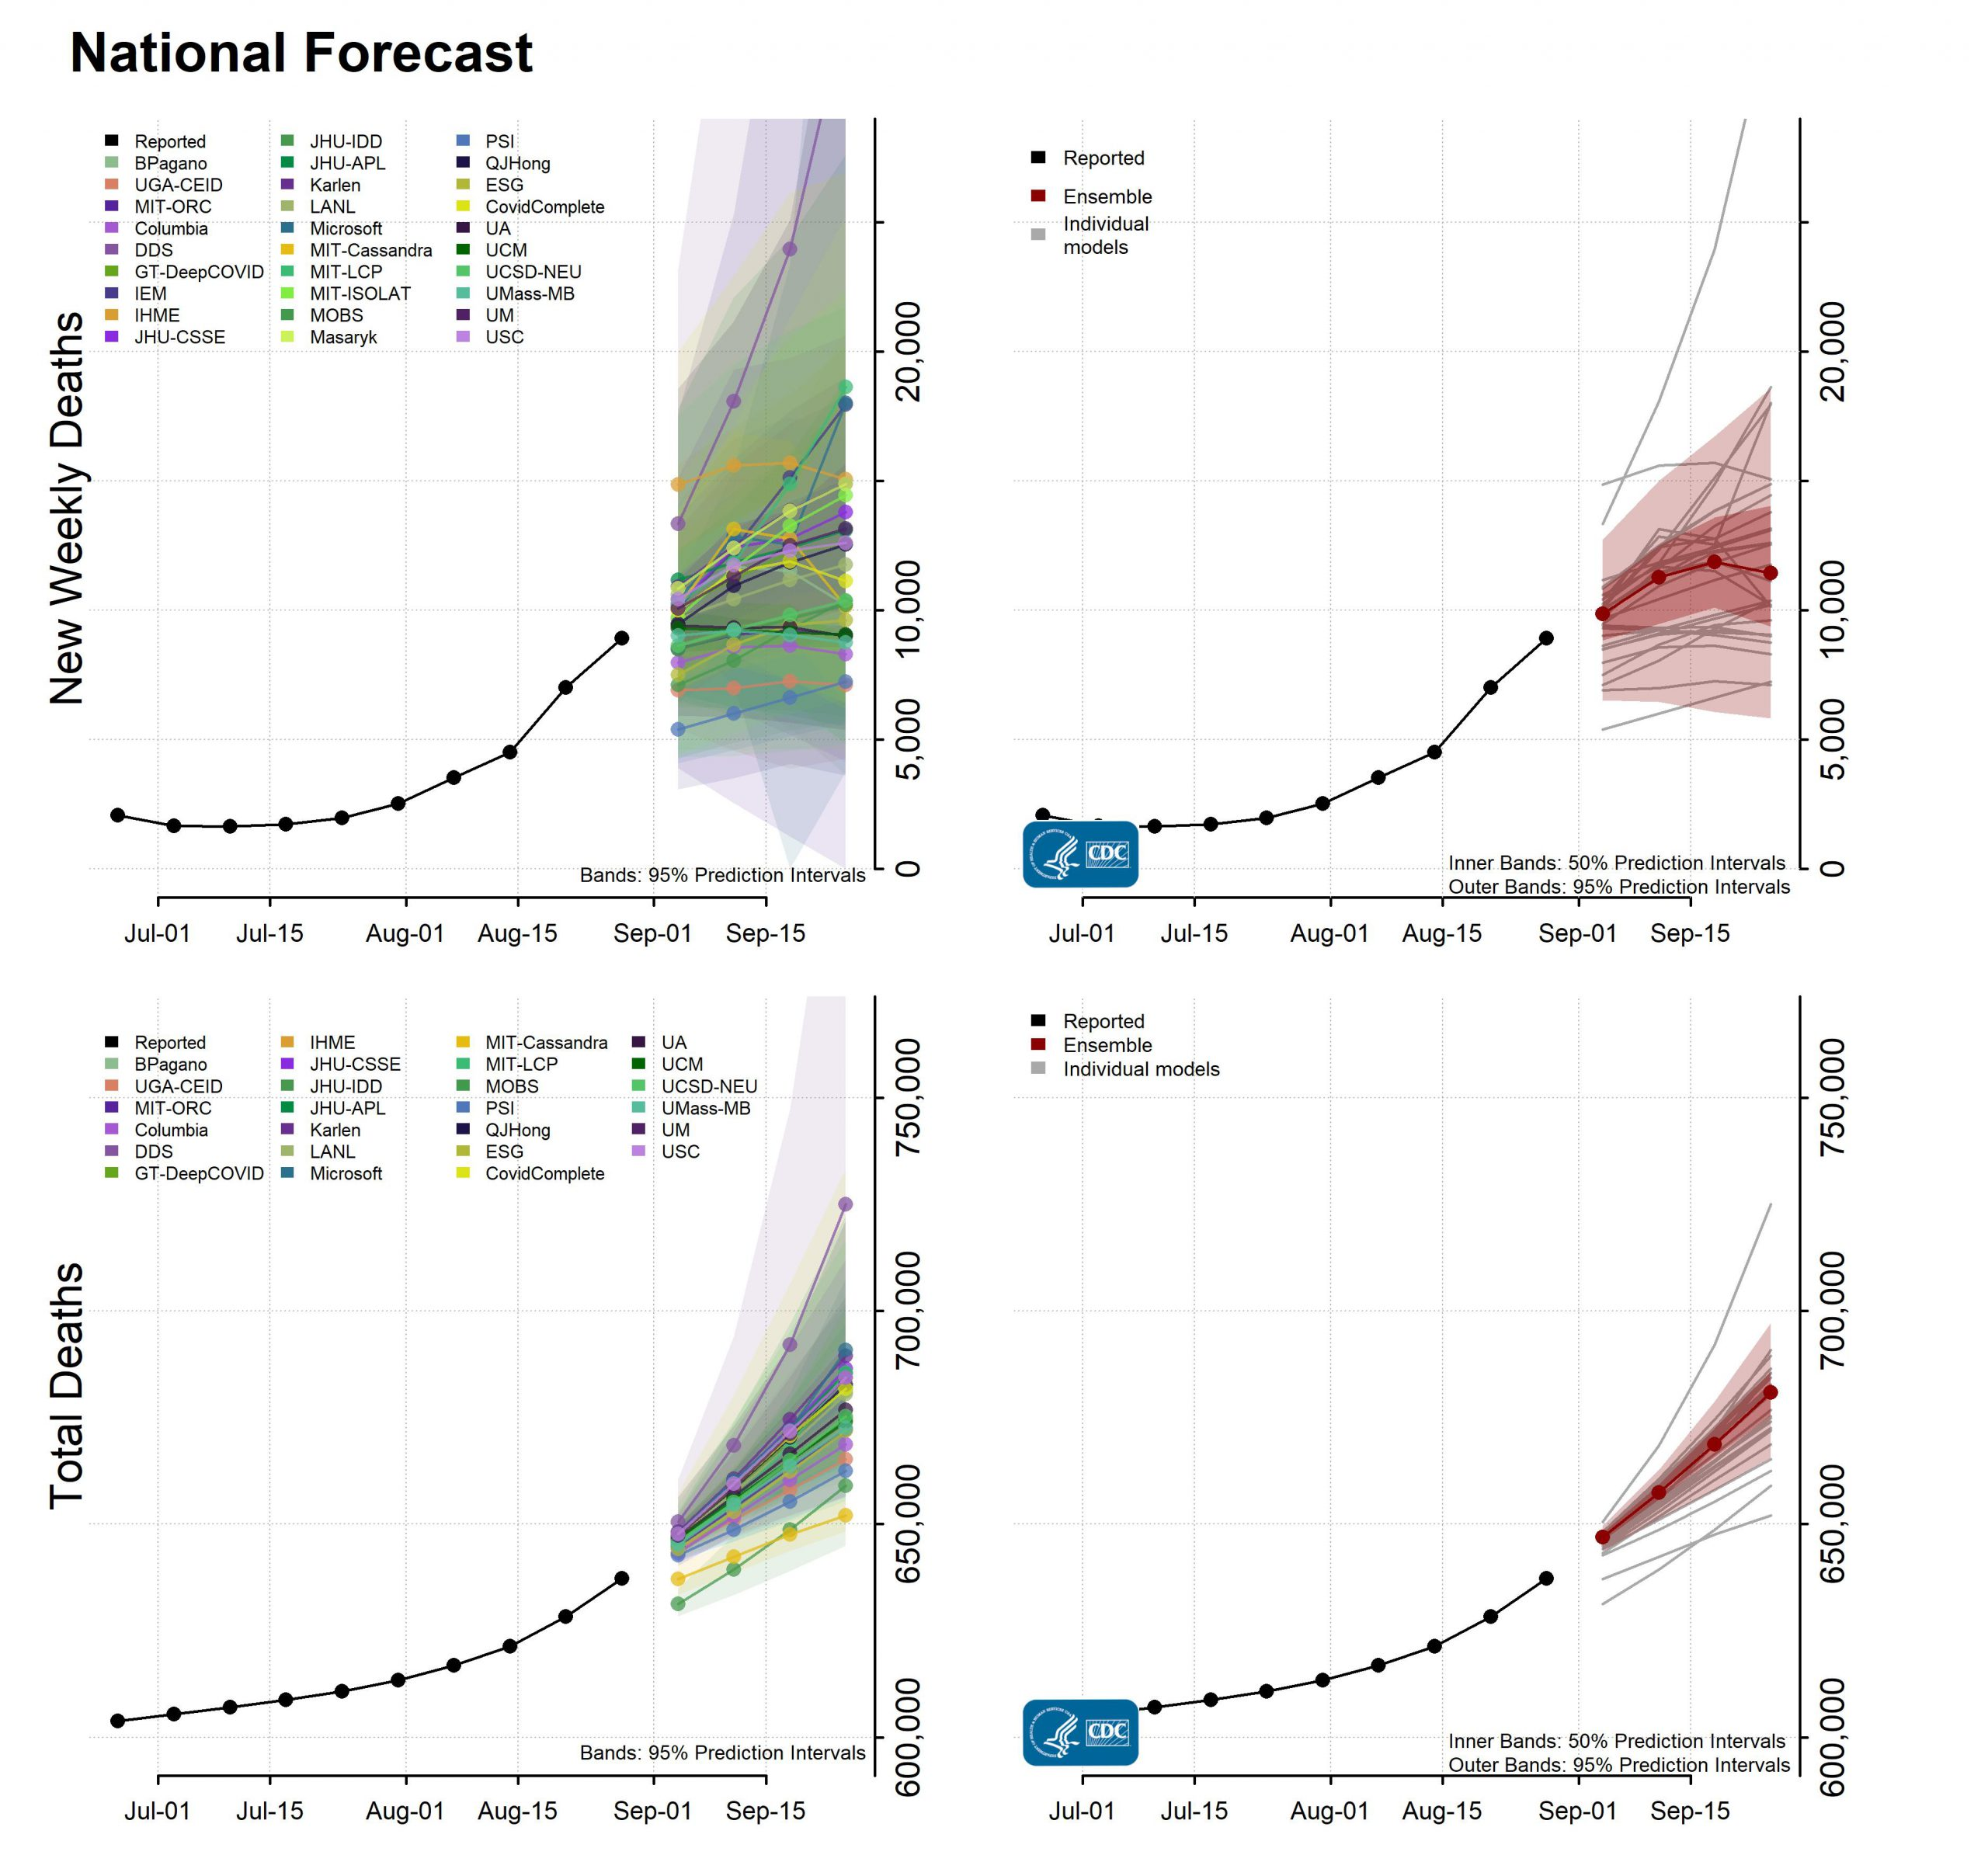
\includegraphics[scale=.12]{8_30_21_cvd_deaths.jpeg}}
\caption{Figure this out later}
\label{fig}
\end{figure}

\subsection{...}
In the context of collaborative forecasting like that of the CDC flu competition
or the COVID-19 Forecast Hub, discretized bins and quantile forecasts have 
proven useful and effective. Yet both types come with their drawbacks. Data 
storage for instance might be a concern if many bins are allowed for a 
prediction. And scoring methods are limited if forecasts are made of quantiles.

In this paper, we propose the use of discrete mixture distributions as a means 
of forecasting for projects similar to the CDC flu competition or the COVID-19
Forecast Hub. In section 2, popular probabilistic forecast representation 
types will be defined and reviewed. Methods of scoring, storing, building 
ensembles and other aspects will be reviewed and compared for each 
representation type.
Section 3 is a retrospective study of the CDC flu competition and COVID-19 
forecast predictions and an attempt to assess whether any predictions 
approximately come from well known continuous distributions.


\section{Probabilistic Forecast Representations}

Before introducing discrete mixture distributions as a candidate for a
probabilistic forecast, we review representations already commonplace in 
forecasting. In a collaborative setting, certain aspects of each representation
should be considered. With each representation presented, 
commmon application of 
scoring, data storage and ensemble construction will be considered for each type
as well as other notable properties.

\subsection{Considerations...}
\subsubsection{Scoring}
Scoring rules are used to evaluate numerically a probability forecast. The
score is a measure on the accuracy of the forecast and where multiple forecasts
exist may provide a rank for each relative to the others. If a scoring rule is 
proper, then the highest possible reward is obtained by reporting the true 
distribution. The rule is strictly proper if that value is unique. 
Under proper
scoring rules, a forecaster has no incentive to be dishonest in their 
submission \cite{gneiting2007strictly}. This makes proper scoring rules ideal
for grading forecasts. We will limit our review of scoring methods to rules
which are proper.

\subsubsection{Storage}
For a forecast hub collecting many predictions, computer storage is something
that needs to be addressed. For a project involving many researchers, the 
number of forecast predictions can add up. For example, the repository for the
COVID-19 Forecast Hub predictions contained 85.4 million predictions as of 
February 5, 2022! (cite zoltar??)
When determining the goals of a forecast project, there should be consideration 
of the storage required for different representations.

\subsubsection{Ensemble Modeling}
A multi-model ensemble is a statistical model made by combining information from
2 or more individual statistical models. Private and public decisions are 
regularly made after combining information from multiple sources. For any given
situation, information from one source may shed light on a subject which other
sources fail to capture. Likewise one statistical model may provide perspective
that another model does not, so that when they are combined in an ensemble the 
resulting model is superior.

As probabilistic forecasting becomes more commonplace, so too does ensemble 
modeling. Multi-model ensembles have been used extensively in weather and
climate modeling see \cite{baran2018combining}, 
and they have been used increasingly in modeling infectious disease outbreaks
see for example \cite{yamana2016superensemble}. 
Multi-model ensembles allow for an incorporation of multiple signals -
often from differing data sources- and for individual model biases being canceled
out or reduced by biases in others (\cite{reich2019accuracy} see references
therein). 
In several disease outbreak studies, multi-model ensemble forecasts have been 
shown to outperform individual model forecasts (\cite{cramer2021evaluation} see
references therein).

Construction of an ensemble may be done by combining individual forecast 
distributions using weighted averages. This has been called stacking 
\cite{wolpert1992stacked} or weighted density ensembles 
\cite{ray2018prediction}. 

\subsection{Representations}
\subsubsection{Parametric distributions}
A parametric distribution is a discrete or continuous probability distribution 
described by a known function $p(x) := p(x|\theta)$ -pmf in the discrete case or 
pdf in the continuous case. $\theta$ is a vector of known or unkown parameters 
contained in a parameter space. 

The value of $p(\cdot)$ evaluated at $x$ is defined as 
$p(x) = P(X = x)$ or the probability that the random variable $X$ takes
on $x$ in the space of the random variable. In the continuous case 
$P(D = x) = 0$ for all $x$, but the probability 
that $X$ falls within an interval $(a,b)$ is calculated as

\begin{equation}
  P(a < X < b) = \int_a^b p(x) dx
\end{equation}

Other functions classified by a parameteric distribution include the cumulative
distribution function (CDF) and the inverse CDF or quantile function. The CDF 
in the continuous case is defined as

\begin{equation}
  F_X(x) = P(X \leq b) = \int_{-\infty}^x p(t) dt
\end{equation}
or in the discrete case 

\begin{equation}
\label{eq:dcdf}
  F_X(x) = P(X \leq b) = \sum_{k=1}^n p(x_k) dt
\end{equation}
where $x_n$ is the largest value of X less than or equal to $x$.
The quantile function is defined as
\begin{equation}
  Q(p) = \inf \{ y \in \mathbb{R} : p \leq F_X(x) \}
\end{equation}
returning a quantile value where $p$ is a given probability $0\leq p \leq 1$.

% \subsubsubsection{Scoring}
For a forecast represented as a parametric function with pmf/pdf $p_m(x)$, 
the accuracy of the forecast may be measured as how likely realized value $x^*$
is to occur. Commonly used proper scoring rules for parametric distributions
include the Logarithmic score (LogS), 
continuous rank probability score (CRPS) \cite{hersbach2000decomposition}
\cite{alves2013ncep} and the interval/Brier 
score \cite{gneiting2007strictly} among 
others. See also \cite{gneiting2014probabilistic}
section 3 for on proper scoring functions. Unless otherwise noted, the following
definitions/reviews can be found in the review by Krueger.

For a forecast with pdf/pmf $p_m(x)$, the Logarithmic score evaluates the 
probability of the observed value $x^*$. It is defined as

\begin{equation}
  LS(p_m,x*) = -log\;p_m(x^*)
\end{equation}
The goal is to minimize the LogS, so that a forecast $p{'}_m(x^*)$ is deemed 
superior to $p_m$ if
$LS(p{'}_m, x^*) < LS(p_m, x^*)$.
The LogS is strictly limited to scoring forecasts with density functions and
evaluating those densities only at the point $x^*$.

The CRPS is a function of a CDF $F$
and so 
can be used a bit more extensively than the LogS which is limited to 
distributions which carry a density. For the CDF $F_m$, the CRPS is defined as

\begin{equation}
\label{eq:crps}
  CRPS(F_m, x^*) = \int_{-\infty}^{\infty} (F_m(x)- 1_{\{x*\leq x\}})^2 dy
\end{equation}
Here too a smaller score indicates a better forecast.

Besides evaluating forecasts, the CRPS is also used in optimizing weights used
to build ensembles. Considered the state-of-the-art techniques for combining 
component distributions
into a multi-model ensemble are nonhomogeneous regression (NR), also known as
ensemble model output statistics (EMOS), and ensemble Bayesian model averaging
(BMA), both of which will be defined as in \cite{gneiting2014probabilistic}.

In the context of an ensemble made from component models submitted from various
sources, contructed with different methods and with potentially different data,
BMA is the better option. In BMA, the final model does not have to be specified
beforehand and the resulting forecast will be a discrete mixture distribution
of all component forecasts. The general form for the ensemble distribution $p^E$
is

\begin{equation}
\label{eq:bma}
  p^E(x) = \sum_{jm=1}^M w_mp_m(x)
\end{equation}
where $p_m$ is the $j^{th}$ component forecast distribution and 
$0 \leq w_m \leq 1$ is a weight assigned to each component where $\sum w_m = 1$.
Methods for estimating weights include Maximum Likelihood estimation
\cite{raftery2005using}, MCMC 
sampling see \cite{vrugt2008ensemble} (also in this paper it talks about how 
EM can get difficult as parameters i.e. number of distributions increase, and 
shows MCMC may be better with that high dimensionality and gives full posterior
of weights)
and minimizing the CRPS as in 
\cite{baran2018combining}.

For selecting distribution weights, the CRPS has some nice properties, but can 
sometimes be
difficult to compute. For example, when the forecast is a mixture of a 
Truncated Normal distribution (TN) and a Truncated Lognormal (TL) the CRPS is 
not available in closed form \cite{baran2018combining}.

Generally computation and evaluation of parametric distributions is not hard. 
For most commonly used parametric distributions -Normal, Lognorm, Poisson,
Gamma, etc.- there is software readily available to compute density, 
distribution and quantile values. Likewise, requirements for storage are low 
compared to other uncertainty representations we will discuss. The most common
parametric distributions can be fully defined with three or pieces of data.
The distribution family and two or three parameters. Below shows a table with
enough information to completely define a $Lognormal(1,0.4)$ distribution.

\begin{table}[h!]
\label{tab:pstor}
\centering
 \begin{tabular}{|c c c|} 
 \hline
 Family & param1 & param2 \\ [0.5ex] 
 \hline
 lnorm & 1 & 0.4 \\ 
 \hline
 \end{tabular}
\end{table}

A completely defined continuous parametric distribution can be evaluated at an
infinite number of values. We will call this an infinite resolution.


A drawback of representing a forecast in a parametric distribution is the lack 
of flexibility in the model selection. Easy computation and evaluation of these 
models is limited to what is available in software, so certain distributional
shapes may unattainable. The distribution may assign probability to values
outside the range of the forecast. There are remedies for this such as 
truncation, but these increase the complexity in evaluation and scoring.
Requiring a parametric forecast also bars the use of some statistical methods
which might be used to create a forecast model including some Bayesian methods
where a posterior distribution cannot be computed in closed form.


\subsubsection{Sample Distributions}
Some forecast model builders may want more flexibility than a parametric 
distribution can provide. Some methods such as sampling from a posterior 
distribution or resampling methods like Bootstrap will produce forecasts of
sample distributions. 

A sample distribution is built of a sample of random variables 
$(X_1,...,X_n)$ where $X_i \sim D$ and $D$ is a distribution. From this, sample
statistics such as mean, median, variance and quantiles may be calculated. 
An empirical cumulative distribution function (ECDF) may also be calculated as

\begin{equation}
\label{eq:ecdf}
  F_n(x) = \frac{1}{n} \sum_{i=1}^n \mathbb{I}(X_i \leq x)
\end{equation}

According to the Strong Law of Large numbers, the sample mean will converge to
the expected value of distribution as $n \rightarrow \infty$ as long as the 
expected value of that distribution exists. Likewise by the same law the 
ECDF will converge to the true CDF 
distribution function as $n \rightarrow \infty$. Thus, if a sufficiently large 
sample is generated from a distribution, the sample will closely approximate the 
true distribution. 

For common distribution families it is easy to generate large samples using 
existing functions in R and other programming platforms. For some distributions 
for which the mathematical formula is unkown or is not in closed form, more 
sophisticated methods may be required to generate samples. Bayesian analyses may 
require a Gibbs or Metropolis-Hastings algorithm, among others, to generate a 
sample. Such samples are useful in that the true distribution may be closely 
approximated without knowing the true mathematical form. 

So the options that a researcher has for constructing a forecast are more than
if they are asked to submit a parametric distribution and the characterisitcs 
and potential shapes of distributions is much larger.
In the last few decades, increased computing power and improvements in MCMC
sampling have greatly contributed to growth in the use of
predictive distributions \cite{gneiting2007strictly}. (See examples listed in
\cite{krueger2016probabilistic}).

To properly score a forecast represented by a sample distribution, both the CRPS
and LogS may be used. The CRPS has the advantage here of scoring the sample 
distribution directly since the CDF in  (\ref{eq:crps}) may be replaced by 
(\ref{eq:ecdf}). To use the LogS to score a forecast, a density function for the 
sample must be approximated. Common approximations include a kernel density (KD)
or Gaussian approximation (GA).

KD is defined in Kruger as

\begin{equation}
\label{eq:kd}
  \hat{p}_n(x) = \frac{1}{n h_n} \sum_{i=1}^n K \left( \frac{x-X_i}{h_n} \right) 
\end{equation}
where $K$ is a kernel function, and $h_n$ is a suitable bandwidth. GA is defined
as 

\begin{equation}
\label{eq:ga}
  \hat{F}_n(x) = \Phi  \left( \frac{x-\hat{\mu}_n}{\hat{\sigma}_n} \right)
\end{equation}
where $\Phi$ is the standard normal CDF and $\hat{\mu}_n$ and $\hat{\sigma}_n$
are the empirical mean and standard deviation of the sample $(X_i)$. (See
\cite{krueger2016probabilistic} for definitions of \ref{eq:kd} and \ref{eq:ga}).

Kruger et. al compare scoring of MCMC drawn forecast distributions using CRPS 
and LogS over samples directly using ECDF or over density approximations using
KD or GA.

To build an ensemble model from sample distribution forecasts, the BMA 
construction from (\ref{eq:bma}) would work only replacing $p_m$ with 
$\hat{p}_{n_m}^{KD}$ or $\hat{p}_{n_m}^{GA}$. Here as well the optimal weights 
$w_m$ may be estimated by maximizing the likelihood or minimizing CRPS. Then 
the ensemble distribution would take the form of a continuous or discrete
probability mixture distribution. If the desire is that the ensemble still be
a sample distribution, after selecting weights, a sample may be selected by 
randomly selecting a sample from $(X_n)_m$ with probability $w_m$.

A potentially big issue with using sample distributions is the amount of storage
it would require. For example when making MCMC draws from a posterior 
distribution, the final sample distribution can have a sample size of thousands
or tens of thousands. Maybe not all distributions would require such a large 
sample size, but sizes of at least dozens or hundreds would be required for each
forecast prediction. For any project the size of the CDC flu competition or the
COVID-19 Forecast Hub, the storage required would be large and potentially 
expensive.

\subsection{Discretized bin distributions}
An alternative to parametric distributions and sample distributions which allows
for high flexibility in distribution shape but is more manageable in terms of 
storage is a discretized bin distribution.

A discretized bin probability distribution may be constructed over a set 
$A = [a, b]$ by partitioning $A$ into a set of $K$ bins $\{B_i\}_{i=1}^{K}$
where $B_i = [b_{i-1}, b_i)$ and $\cup_{i=1}^{K} B_i = A$. Based on the problem
to be forecasted, a forecast hub will determine the possible values for $A$ and 
select the number of bins and the sizes for each. It may be the case
that a forecast hub will set the width of all bins to be equal so that 
$\Delta = b_i - b_{i-1}$ is the width for all $i$ see for example
\cite{mcgowan2019collaborative}.
To complete the construction, a probability $p_i$ is assigned to each $b_i$ 
where $\sum_{i=1}^{K}p_i = 1$. These probabilities are determined by the 
forecasters. 
This discrete representation with a given bin and assigned probability is in
essence a probability mass function in that the calculation of moments and the 
the cumulative distribution are done the same as for a discrete parametric 
distribution. For a random variable X from a binned distribution to calculate
the $j^{th}$ moment we may use

\begin{equation}
\label{eq:bev}
  EX^j = \sum_{i=1}^n \beta_i^j p_i
\end{equation}
where $\beta_i$ is a value related to the bin $B_i$ such as $\beta_i = b_i$,
$\beta_i = b_{i-1}$ or $\beta_i$ is the mean or mid value in $B_i$. The 
cumulative distribution may be

\begin{equation}
\label{eq:bcdf}
  P(X \leq b) = \sum_{i=1}^n p_i
\end{equation}
where $p_n$ is the probability for the bin $B_n$ where $b \in B_n$.

If the value to be forecasted takes on discrete values, a common discrete 
distribution, such as a binary or Poisson distribution, may sometimes be used to 
assign probabilities to each of the bins. When the values to be forecasted are
continuous, a forecaster may need to employ a method of discretization to a 
forecast distribution. There are a number of possible ways to do this including
those outlined by Chakraborty and Subrata \cite{chakraborty2015generating}.

The CDC has used a discretized distribution representation as the representation
for their annual influenza forecasting competition and other disease outbreaks.
In that context it has become the standard representation 
\cite{brooks2020comparing}. A decent amount of work has been done in evaluating 
and constructing ensemble models on influenza forecasts represented by 
discretized bins \cite{mcgowan2019collaborative}, \cite{mcandrew2019adaptively}
\cite{reich2019collaborative}. 

Because discretized bins can be seen as a pmf, methods for proper scoring 
already 
discussed -LogS and CRPS- are useable and BMA is valid method for ensemble 
construction. Reich et. al used BMA to combine multiple forecasts from the flu 
competition. There built and compared ensemble models with different weighting
schemes including equally weighted components $w_j = 1/J$ and estimating weights
according to the model specification. To estimate weights they used the 
Expectation Maximization (EM) algorithm \cite{reich2019accuracy}. See the
supplementary material for details. 

The exact amount of information required for a discretized bin forecast will 
vary depending on permitted range of the forecast and the desired resolution. 
In the CDC flu contest, a forecast could have 131 bins between 0\% and 13\% 
-bins having increments of 0.1- with 
corresponding probabilities in each. That makes 262 pieces of information per
prediction. For any binning scheme of more than two bins, the information 
requirement for discretized bins will be higher than for parametric distrbutions.
Table \ref{tab:dbins} illustrates what a discretized 
Lognormal$(1,0.4)$ distribution truncated over $[0,8]$
looks like in 41 equally spaced discretized bins. The discretization was done
such that 

\begin{equation}
\label{eq:disc}
  p_i = \int_{b_{i-1}}^{b_i} p^{TL}(x) dx
\end{equation}
where $p^{TL}$ is the pdf of a truncated Lognormal$(1,0.4)$. This is similar
to Methodology-IV from Chakraborty \cite{chakraborty2015generating}
 \cite{kemp2004classes}.

\begin{table}[h!]
\label{tab:dstor}
\centering
 \begin{tabular}{|c|c|} 
 \hline
    bin & prob \\ \hline
    ... & ... \\
    {[1.4,\;1.6)} & 0.04414 \\
    {[1.6,\;1.8)} & 0.05896 \\
    {[1.8,\;2.0)} & 0.07032 \\
    {[2.0,\;2.2)} & 0.07172 \\
    {[2.2,\;2.4)} & 0.07955 \\
    ... & ... \\
 \hline
 \end{tabular}
\end{table}
Submitted as a forecast prediction, the distribution in table \ref{tab:dstor} 
includes 82 pieces of data. For parts 
of the CDC influenza competition some forecasts included upt to 262. This is 
much more manageable than possible thousands of samples from a samle 
distribution but is 
still much larger than the 3 or 5 data pieces required to report a lognormal
or truncated lognormal distribution.

Depending on what is known about the problem to be solved, creating the right 
binning scheme might be a challenge. Because there must be a finite number of
bins, forecast distributions must have a finite support. Where the range of 
possible outcomes to a problem is little known, the right binning scheme may be
hard to produce.









\subsection{Quantile representation}
When deciding how forecasts should be represented in the COVID-19 Forecast Hub,
the time pressure of generating forecasts and the consideration of the large
range for possible outcomes contributed to the COVID-19 Forecast Hub decision
to forego trying to create the right binning scheme and use sets of prediction
intervals to represent uncertainty in predictions \cite{bracher2021evaluating}.

The Forecast Hub requires predictions to be submitted as 11 or 3 nominal 
intervals -depending on the specific target- and a median.
Using this interval or quantile representation lead to a number of changes in 
the evaluation and aggregation of forecasts.

A quantile forecast is constructed as follows.
For $N$ given quantiles $\alpha_1,..., \alpha_N$, $q_1,..., q_N$ are the values
such that 

\begin{equation}
  P(Y \leq q_1) = \alpha_1, P(Y \leq q_2) = \alpha_2, ..., 
  P(Y \leq q_N) = \alpha_N
\end{equation}
When the quantiles are reported as prediction intervals we have more 
specifically

\begin{equation}
  P(Y \leq q_1) = \alpha_1, P(Y \leq q_2) = \alpha_2, ...,
  P(Y \leq q_{N-1}) = 1 - \alpha_{N-1}, P(Y \leq q_N) = 1 - \alpha_N
\end{equation}

The quantile or interval format is somewhat unique among forecast 
representations discussed in this paper. What is possible for scoring forecasts
or building ensemble models in other representations is often not possible with
quantile forecasts. The shape of a distribution is also not known and in fact,
nothing is known about the tails of the uncertainty or ouside of the most 
extreme reported quantile values. In the Forecast Hub predictions, nothing 
is said about the range below the $1^{st}$ quantile or above the $99^{ths}$.
Yet the quantile representation has its advantages. 

Quantile representation allows for forecasters to submit fairly detailed
forecasts without restricting the range of possible values.
Since quantiles are easily calculated from any regular distribution type
-e.g. quantile function for parametric functions or calculating sample 
quantiles- we consider quantile forecasts to have high flexbility in terms of 
what methods forecasters may employ in modeling.

To score predictions from a prediction interval, 
neither the LogS nor the CRPS may be used, 
but another proper scoring rule the interval score (IS) may be.
For an observed outcome $x^*$ and a prediction interval $(l,r)$ 
where $l$ and $r$ are the $\alpha/2$ and $(1-\alpha/2)$ quantiles that bound
the central $(1-\alpha)$ prediction interval the IS is defined as

\begin{equation}
\label{eq:is}
  IS_{\alpha}(l,r; x^*) = (r-l) + \frac{2}{\alpha}(l-x^*)1\{x^*<l\} 
  + \frac{2}{\alpha}(y-r)1\{x^* > r\}
\end{equation}
This is a sum -weighted by 
$\alpha$- of the width of the
interval and the distance between $x^*$ and the interval (if $x^*$ is not 
captured in the interval) \cite{gneiting2014probabilistic}. 
The IS requires only a single central 
$(1-\alpha) \times 100$ prediction interval.

When an interval forecast is made up of more than one interval with different
$\alpha$ levels, a weighted interval score (WIS) may be evaluated. Bracher et.
al use the WIS to evaluate COVID-19 inverval forecasts 
\cite{bracher2021evaluating}.
There are multiple versions of the WIS -some of 
which are described by Bracher et. al- but that used in the COVID-19 Forecast
Hub is defined as follows

\begin{equation}
  WIS_{0,K}(F_m,y^*) = \frac{1}{K + 1/2} \times (w_0, \times |y^*-med|+
  \sum_{k=1}^K \{ w_k \times IS_{\alpha_k}(F_m,y) \} )
\end{equation}
$w_k = \alpha_k/2$ is the weight on
intervals which was used. With that choice of weights, it may be shown that the
WIS approximates CRPS see S1 Text  \cite{bracher2021evaluating}

Bogner, Liechti and Zappa compared scoring forecasts of quantiles with the 
Quantile Score similar to the interval score and scoring distribution functions
fit to those quantiles using CRPS \cite{bogner2017combining}. The CRPS 
corresponds to the integral of the QS over all possible thresholds rather than
just specific quantiles, it more effectively reveals deficiencies in parts of 
the distribution and especially in the tails past the end points of quantiles
used in QS or IS.

Like the CRPS, not only does the WIS provide an easily interpretable proper 
score for interval forecasts, but it may also be useful when building an 
ensemble forecast.

The ensemble forecast constructed by the COVID-19 Forecast Hub was made as an
equally-weighted average of forecasts from the component models. More 
specifically, each quantile value of the ensemble was the average of values from
all models corresponding to the same quantile \cite{ray2020ensemble}. For $M$ 
models each with $K$ quantiles, the $k^{th}$ ensemble quantile $q_k$ is 
calculated as

\begin{equation}
\label{eq:qa}
  q_k = \sum_{m=1}^M \nu_m q_k^m 
\end{equation}
where $\nu_m$ is the weight assigned to each forecast and $\sum \nu_m = 1$. In
the Forecast Hub model, $\nu_m = \nu = 1/M$. Where the overall mean or a
weighted mean may be used, the median may also be used.
Brooks et. al compare performance of the COVID-19 ensemble
between equally-weighted means, weighted means and median value constructions.
\cite{brooks2020comparing} (is is appropriate to cite this blog??)
In their report, they show that weighted means and median constructions tend
to outperform equally-weighted mean construction. To come up with optimal 
weights, they select values $\nu_m$ from \ref{eq:qa} which minimize the WIS of 
the ensemble forecast.

Averaging quantiles in this way the same as quantile averaging or Vincentization
only with an incomplete quantile function. It thus carries with it many of the
same characteristics.
Quantile averaging or Vincentization for a complete distribution is defined as 

\begin{equation}
\label{eq:vinc}
  F_v^{-1}(\alpha) = \sum_{m=i}^M w_m F_m^{-1} (\alpha)
\end{equation}
where $F_m^{-1} (\alpha) = \inf \{y:F_m(y) \geq \alpha\}$ for 
$0 < \alpha \leq 1$. Some notable characteristics are that it is more likely
to be unimodal than linear averaging of densities like BMA 
\cite{busetti2017quantile} (this paper is a comparison of QMA and 
linear or log averaging. Under some circumstances, such as when member
distributions are exponential, Weibull or logisitic the aggregated distribution
is the same \cite{ratcliff1979group}. It produces smoother
distributions than BMA according to Schepen and Wang \cite{schepen2015model}.
Lichtendahl et. al conclude that quantile averaging produces sharper forecasts
and tends to perform better in scoring than probability averaging
\cite{lichtendahl2013better}.

As in sample distributions and binned distributions, 
data storage for interval forecasts will
depend on the desired clarity of resolution. For the COVID-19 forecasts 
submitted to the forecast hub, twenty-three quantile values are requested for 
the quantiles (0.01, 0.025, 0.05, 0.10, …, 0.95, 0.975, 0.99). This included a 
median along with eleven confidence intervals \cite{bracher2021evaluating}. This
requires forecasters to submit forty-six values in each short-term forecast 
(some of the longer term forecasts only include seven quantiles). In terms of 
storage, this is an improvement over requirements for the flu contest. Table
\ref{tab:qstor} shows what a submission of 23 quantiles from a 
Lognormal $(1,0.4)$ looks like.



% \begin{table}[h!]
% \centering
%  \begin{tabular}{|c|c|} 
%  \hline
%     quantile & value \\ \hline
%     0.01 & 1.07137 \\
%     0.025 & 1.2404 \\
%     0.05 & 1.40689 \\
%     0.01 & 1.62675 \\
%     ...  & ... \\
%     0.9 & 4.50667 \\
%     0.95 & 5.18328 \\
%     0.975 & 5.82391 \\
%     0.99 & 6.58783 \\
%  \hline
%  \end{tabular}
% \end{table}

\begin{table}[h!]
\centering
\label{tab:qstor}
 \begin{tabular}{|c|c|c|c|c|c|c|c|c|c|}
 % \begin{tabular}{|c|c|}
 \hline
    quantile & 0.01 & 0.025 & 0.05  & ...  & 0.95 & 0.975 & 0.99 \\ \hline
    value & 1.07137 & 1.2404 & 1.40689 & ... & 5.18328 &
    5.82391 & 6.58783 \\
    % quantile & value \\ \hline
    % 0.01 & 1.07137 \\
    % 0.025 & 1.2404 \\
    % 0.05 & 1.40689 \\
    % 0.01 & 1.62675 \\
    % ...  & ... \\
    % 0.9 & 4.50667 \\
    % 0.95 & 5.18328 \\
    % 0.975 & 5.82391 \\
    % 0.99 & 6.58783 \\
 \hline
 \end{tabular}
\end{table}


\begin{figure}[htbp]
\centerline{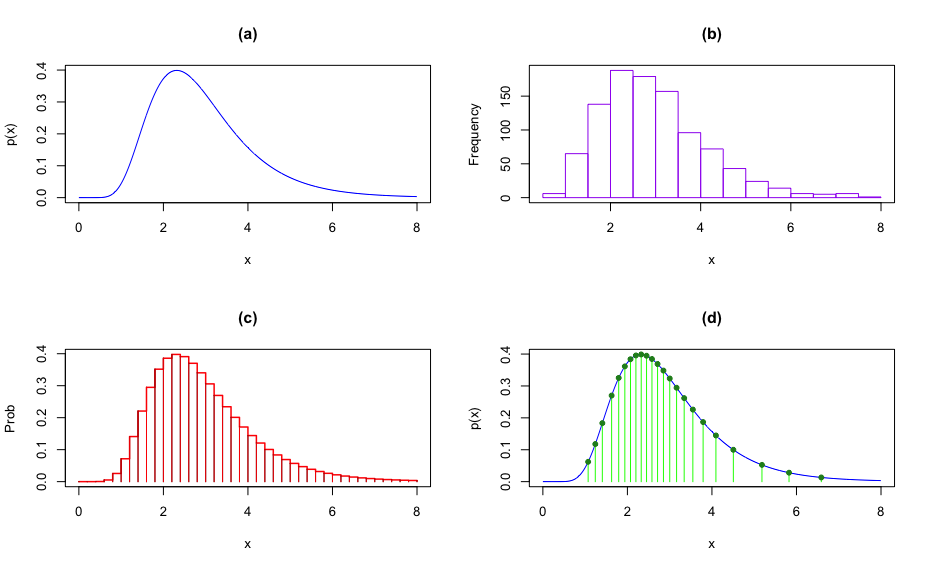
\includegraphics[scale=.4]{dens_comp.png}}
\caption{Figure this out later}
\label{fig}
\end{figure}

\begin{figure}[htbp]
\centerline{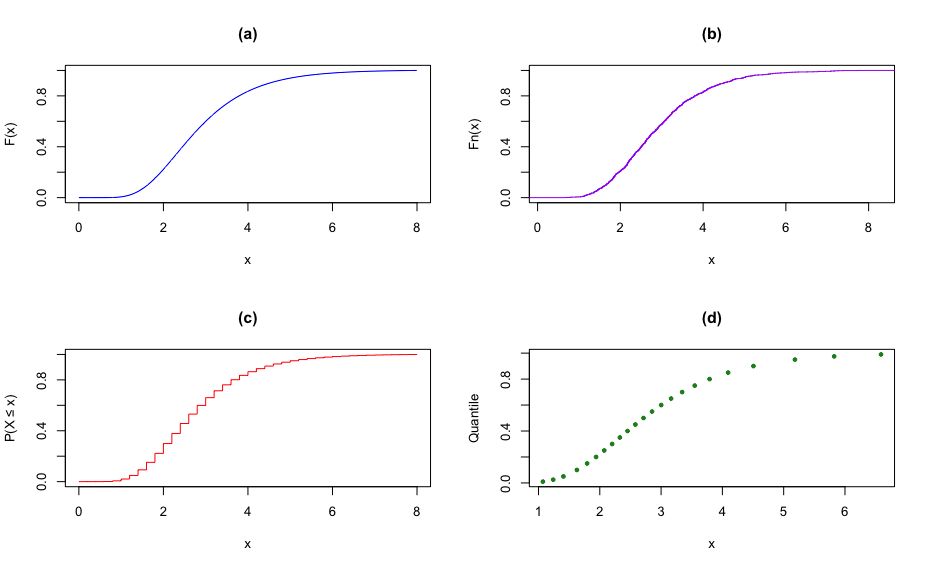
\includegraphics[scale=.4]{cum_comp.png}}
\caption{Figure this out later}
\label{fig}
\end{figure}



\subsection{Discrete mixture of parametric distributions}
In a parametric setting, forecasters may be permitted to submit a forecast as a
discrete mixture. Such a distribution may be constructed in the same way as the
ensemble described under Parametric distributions (\ref{eq:bma}) 
where for $T$ distributions
with pdfs $p_t(x)$ and $z_t > 0$ and $\sum_{t=1}^{T} z_t = 1$
 

\begin{equation}
\label{eq:dmd}
  p^{M} = \sum_{t=1}^T z_tp_t(x)
\end{equation}




Like the standard parametric model, a discrete mixture is easily evaluated with
exisiting software (like distr R package \cite{camphausen2007distr}). And 
scoring may be done by 
using the LogS, CRPS and IS. The resolution of a discrete mixture is high 
and the support need not be limited by submission requirements. 

A mixture distribution may be much more flexible than a simple parametric in 
terms of distributional shape. But as it is essentially parametric, forecasters
mays still be limited in how they construct their models. But it may be possible
to fit a mixture distribution to probability models with the other 
representations discussed. According to McLachlan and Peel, a finite mixture of 
normal densities with common variance can be used to approximate abitrarily well
any continuous distribution \cite{peel2000finite} (see also 
\cite{nguyen2019approximations}). Thus, for any unconventional probability
distribution -such as MCMC posterior samples- it may be reasonable to 
approximate the distribution by a mixture of normals.
Further discussion on methods for fitting mixture 
distributions to different types of model representations is included in this 
paper.

An ensemble model may be built by using (\ref{eq:bma}) only replacing $p_m$
with $p^M$. Solving for weights may also be done similarly, though with the 
added complexity of component models being mixture distributions, the 
computation is likely to get more expensive. An example where this may be
especially true is when minimizing of CRPS, but the exact mixture doesn't 
result in CRPS in closed form \cite{baran2018combining}.

Depending on the number of components a forecaster includes in a mixture 
forecast, the amount of storage per forecast might be as little as for a 
parametric forecast and as much as a forecast hub will allow. For modelers whose
models produce distributions with irregular shapes, it may be that those
distributions can be closely approximated by the right mixture distribution.




\begin{flushleft}
    \begin{adjustwidth}{-3cm}{-1cm}
    \begin{tabular}{ | p{2.4cm} | p{3cm} | p{4cm} | p{3cm} | p{3.5cm} |}
    \hline
    Representation & Scoring & Flexibility/Information & Ensemble &
    Storage Requirement
    \\ \hline

    Parametric & LogS, CRPS, IS & Limited to common distribution families. 
    Infinite resoution
    & BMA & Low 3-6 values/prediction \\ \hline
    
    Samples & CRPS and IS. LogS after smoothing & Any shape. Resolution may be
    high but depends on sample size & BMA after smoothing. Resampling otherwise& 
    Hundreds or thousands of values/prediction
    \\ \hline
    
    Discretized bins & LogS, CRPS, IS &
    Any shape allowed, but limited by binning scheme & BMA &
    Depends on binning scheme but dozens to hundreds of values
    \\ \hline


    Quantiles & IS, WIS & Shape unknown but may still have much info with 
    enough quantiles. No tail information & Quantile averaging & Depends on 
    quantiles requested but dozens of values
    \\ \hline
    
    Discrete Mixture & LogS, CRPS, IS. May be more limited by computation & Can
    take on many shapes/approximate most & BMA 
    & 3 to limit values permitted
    \\ \hline

	 \end{tabular}
	 \end{adjustwidth}
\end{flushleft}

% bin & -6.5 & -6.4 & -6.3 $ ... & 6.3 & 6.4 & 6.5 \\  
%  prob & 3.75e-11 & 1 7.11e-11 & 1.33e-10 & ... & 7.11e-11 & 3.75e-11 & 1.96e-11\\

\newpage


\section{Retrospective Analysis}

\subsection{CDC Influenza like Illness}
The CDC Retrospective Forecasts project at zoltrdata.com (cite??) contains over
850,000 probabilistic ILI predictions for all combinations of of eleven regions 
in the United States and seven targets from twenty-seven different models. These
include predictions during Influenza season between October 2010 and December
2018. All predictions are in the form of discretized probability bins. 

We wanted to determine whether or not some or any of these binned forecasts may
have come from known continuous distribution families such as Uniform, Normal, 
Lognormal or Gamma families. The process we followed for making such a claim was
to "fit" a distribution to the probabilities provided in the forecast by
minimizing

\begin{equation}
  \sum_{i=1}^K (p_i - [F(b_i; \theta) - F(b_{i-1}; \theta)])^2
\end{equation}

Here $F(\cdot; \hat{\theta})$ is a CDF, $p_i$ is the reported probability for 
the $i^{th}$ bin $B_i := [b_{i-1}, b_i)$ and $K$ is the number of bins.
The fitted parameter vector $\hat{\theta}$ is the solution to 

\begin{equation}
\arg\min_{\theta}\sum_{i=1}^K (p_i - 
[F(b_i; \theta) - F(b_{i-1}; \theta)])^2
\end{equation}

If well known continuous distribution was fit to the submitted binned prediction
and the mean sum of squared differences fell below a specified cutoff value, we
considered that the binned predictions were plausibly discretized from the 
continuous distribution.


To determine what values to use as cutoffs we conducted a study where 
binned distributions were discretized from known continuous distributions, 
parameters were fit to the binned distrubtions and the mean sum of squared 
differences was calculated.

For each of Uniform, Truncated Normal (TN), Truncated Lognormal (TL) and 
Truncated Gamma (TG) distributions the following was
done 1,000 times. A set of 131 bins with interval lengths of 
0.1 between 0 and 13.1 was constructed. 
A value $\mu$ was selected from a $Uniform(a,b)$ distribution and $\sigma$ from 
a $Uniform(.05,1.6)$ distribution. $\mu$ and $\sigma$ were taken as respectively 
the center and scale parameters of a TN distribution. 
For Uniform, TL and TG family
distributions, model parameters were solved for so that $\mu$ and $\sigma$ 
were roughly the mean and standard deviation. The minimization was done using 
the `optim` function in the R `stats` package.
Had we accounted for the changes
in moment values from the truncation, the means and standard deviations could 
have been exactly $\mu$ and $\sigma$. But we considered the differences small 
enough that it didn't matter for our purpose.

With a known distribution, probabilities $p_i =F(b_i; \theta) - F(b_{i-1})$ were
calculated for each bin. A Uniform or truncated distribution from the same
family was fit to the bins by minimizing (equation number) with the resulting
distribution function $F(\cdot; \hat{theta})$. From the fitted distribution
$\hat{p_i} = F(b_i; \hat{\theta}) - F(b_{i-1}; \hat{\theta})$ was computed for 
each of the 131 bins. Finally the mean sum of squared probability differences
$\frac{1}{K}\sum_{i=1}^K (\hat{p_i} - p_i)^2$ was calculated. Table (table number)
below shows MSD value for which 95\% of all 1,000 MSDs fell below. Other than in
the case of the Uniform distribution family, those values were selected as the 
cutoff values for declaring whether or not a binned distribution was discretized
from a common continuous distribution.


\begin{table}[h!]
  \centering
  \begin{tabular}{l*{6}{c}r}
  Distribution          & Mean Square Difference 95\%  \\
  \hline
  Uniform               & 8.809460e-05   \\
  Truncated Normal      & 1.126683e-07  \\
  Truncated Lognormal   & 3.877829e-06  \\
  Truncated Gamma       & 1.500152e-06  \\
  \end{tabular}
\end{table}




Of the 869,638 predictions from the CDC Retrospective Forecast project, we fit
each of Uniform, TN, TL and TG distributions to 11,715 of the individual 
predictions. The MSD between the prediction probabilities and the fit
discretized probabilities was calcuated. For each prediction, the fitted 
distribution with the lowest MSD was considered the best fit and if the MSD fell
below the corresponding cutoff value listed in (table number) we consider that 
the prediction approximately follows the fit distribution. The results for the
11,715 fit distributions are seen below.

\begin{table}[h!]
  \centering
  \begin{tabular}{l*{6}{c}r}
  Distribution Family   & Total    & Total Below MSD Cutoff \\
  \hline
  Uniform               & 896      & 669    \\
  Truncated Normal      & 3,804    & 198    \\
  Truncated Lognormal   & 4,501    & 1,340  \\
  Truncated Gamma       & 2,514    & 295    \\
  \end{tabular}
\end{table}

\subsection{COVID-19 Forecast Hub}

As of January 24, 2022 there were nearly 85,000,000 prediction distributions 
from 114 different models submitted to the COVID-19 Forecast Hub (cite??). These 
distributions covered all combinations of 3,202 municipalities (mostly counties) 
in the United States with 441 targets. The first of these forecasts was 
submitted in March of 2020 shortly after the initial outbreak of the virus in 
the US and forecasts had been received weekly since. The forecast representation
for these predictions is the quantile representation where a point estimated is
submitted along with a number of confidence intervals -three or eleven for most
targets. So the predictions typically include seven or twenty-three quantiles.

To assess whether or not a quantile based forecast was formulated from a well
known continuous distribution, we minimized the MSE between the cumulative
density function and the given quantiles. The estimated parameters are the 
solution to $argmin_{\theta} \sum_{i=1}^m (q_i - F(y; \theta))$ where $q_i$ is
the $i^{th}$ given quantile value and $F(y; \theta)$ is the CDF with parameter
$\theta$. This least squares estimating is a more common way to fit a model but
other methods have been presented including Bayesian Quantile Matching
\cite{nirwan2020bayesian}, step interpolation with exponential tails 
\cite{quinonero2005evaluating}
and the Method of Simulated Quantiles 
\cite{dominicy2013method}.

For each prediction used, we fit the quantiles to a Uniform, Normal, Lognormal,
Gamma and Location-scale T CDF. We included the T distribution in case of any
symmetric forecasts with tails heavier than in a Normal distribution.

If the MSE between a given forecast and a fit CDF fell below a certain cutoff,
we considered the quantiles as approximately coming from the fit CDF. To
determine the cutoff values, for each of the five distribution families the same
procedure was followed 1,000 times. 

A decision was made on creating a quantile distribution with 7 quantiles or 23
quantiles with probabilities 1/3 and 2/3 respectively. This was done because 
in the COVID-19 Forecast Hub certain targets require 7 quantiles and others 
require 23. After that decision was made, a random value $\mu$ was drawn from
a $Uniform(2,000,\; 25,000)$ distribution and another value $\sigma$ was drawn
from a $Uniform(3, 200)$ distribution. These values were taken as the mean and
standard deviation and for each of the distribution families considered, the
proper transformations computed to find model parameters corresponding to the 
distribution. Quantile values were calculated for each quantile. When using an 
LST distribution, a value for degrees of freedom was drawn from a 
$Uniform(2,35)$ distribution. A CDF
was fit by minimizing $\sum_{i=1}^m (q_i - F(y; \theta))$ over the parameter
vector $\theta$ and the MSD value $\sum_{i=1}^m (q_i - F(y; \hat{\theta}))$ was 
calculated. The MSD value for which 95\% of the 1,000 simulated distributions
fell below was considered the cutoff and is seen in the table below.

\begin{table}[h!]
  \centering
  \begin{tabular}{l*{6}{c}r}
  Distribution          & Mean Square Difference 95\%  \\
  \hline
  Uniform               & 7.220667e-07   \\
  Normal                & 3.097645e-05  \\
  Lognormal             & 1.166775e-07  \\
  Gamma                 & 2.953370e-05  \\
  Location-scale T      & 0.4894471 \\
  \end{tabular}
\end{table}


With these cutoff values selected, models were then fit to quantile forecasts
from the COVID-19 Forecasts on zoltardata.com. This was a computationally more
difficult problem than fitting distributions to the binned forecasts of the 
influenza project, so the number of predictions fit is much smaller. The 
predictions fit were selected from each of the 115 models with model weeks, 
targets and units selected randomly. In total 2,504 predictions were fit to each
of the five distributions, the MSE was calculated for each and the fit with the
lowest MSE was selected as the closest fit. If the MSE fell below the cutoff
specified above, we considered that the quantile prediction was approximately
from the same distribution as the fit distribution. The results are below.


\begin{table}[h!]
  \centering
  \begin{tabular}{l*{6}{c}r}
  Distribution Family   & Total    & Total Below MSD Cutoff \\
  \hline
  Uniform               & 239      & 0        \\
  Normal                & 609      & 74       \\
  Lognormal             & 694      & 0        \\
  Gamma                 & 597      & 0        \\
  Location-scale T      & 365      & 25       \\
  \end{tabular}
\end{table}

\section{...}



The CDC and the COVID-19 Forecast Hub as well as other collaborative projects
have their own established systems for receiving, 
evaluating and constructing ensemble forecasts. A transition from using binned 
distributions or quantile forecasts to using mixture distributions would require
a few adjustments to those systems. In this section we outline how some of these
adjustments may be implemented as well as present some tools which may be used
to evaluate forecasts and construct ensemble forecasts from multiple models.

\subsection{Submission format}
For a collaborative forecast project to run smoothly, model submissions from all 
modelers should all follow the same format. For both the CDC flu forecasting and
the COVID-19 Forecast Hub, teams are provided a csv spreadsheet with columns 
similar to those in tables \ref{tab:dstor} and \ref{tab:qstor}. Additionally
columns for Location, Target, Type and Unit are included which serve as
indicators of the specific prediction. The values for all variables except 
Value come from a specified list from the forecast center. Value is the 
probability assigned to a bin when the Type is Bin.

\begin{table}[h!]
\label{tab:dstan}
\centering
 \begin{tabular}{|c|c|c|c|c|c|}
 \hline
    Location & Target & Type & Unit & Bin & Value  \\ \hline
    US National & Season Onset & Point & week & NA & . \\
    US National & Season Onset & Bin & week & 0.0 & . \\
    US National & Season Onset & Bin & week & 0.1 & . \\
    ... & ... & ... & ... & ... & ... \\
 \hline
 \end{tabular}
\end{table}

For the quantile forecasts of the Forecast Hub, the possible values for Type 
are Point and Quantile, and rather than using a Bin variable Quantile is used
with values specified by the Hub. Then Value rather than a probability is the
forecasted value for the specified quantile. Per prediction there may be a 
couple dozen rows, up to 24 in the Forecast Hub, or over 100 rows as in some
flu forecasts. 

An adjustment may be made to the format of table \ref{tab:dstan} where each row
represents a compnonent in a mixture distribution.
The variables Bin/Quantile and Value are removed and replaced with Family,
Param1, Param2, Param3 and Weight where Family is the distribution family,
Params are the parameters for the component distribution and Weight is the 
weight $w_i$ for that component.

\begin{table}[h!]
\label{tab:mstan}
\centering
 \begin{tabular}{|c|c|c|c|c|c|c|c|c|}
 \hline
    Location & Target & Type & Unit & Family & Param1 & Param2 & Param3 & Weight
    \\ \hline
    US National & Season Onset & Dist & week & norm & mean & sd & NA & .  \\
    US National & Season Onset & Dist & week & lnorm & meanlog & sdlog & NA & . \\
    ... & ... & ... & ... & ... & ... & ... & ... & .\\
 \hline
 \end{tabular}
\end{table}

A forecast center may want to limit the number of components allowed per 
prediction. For a reference, a mixture distribution prediction with 16 
components would require $16 \times 9 = 144$ cells submitted. This is the same 
number of cells
submitted for a Forecast Hub forecast with 23 quantiles and a point prediction.

\subsection{Mixture construction and scoring tools}

From a submitted forecast, a prediction may be found by Location, Target and 
Unit (or whatever other indication variables are used) and evaluated. We found
the \texttt{distr} \cite{camphausen2007distr}
useful for constructing a mixture distribution given
information like that from table \ref{tab:mstan}. 

The function 
\texttt{UnivarMixingDistribution} takes as arguments a list of distributions
and a vector of weights for each distribution and a object pf a class called 
\texttt{AbscontDistribution} is returned. Functions for density, distribution
and quantile functions as well as for random sampling may then be used on the
mixture distribution object for evaluation. Using those functions and the 
created object, LogS and CRPS are easily calculable. 

We wrote a function \texttt{MakeDist} which takes on a data frame with variables
Family, Param1, Param2, Param3 and Weight and returns a mixture distribution 
of component distributions specified in the rows. 

\subsection{Ensemble construction}

To construct an ensemble distribution from multiple mixture distributions, the 
\texttt{UnivarMixingDistribution} is again a useful tool. Two or more 
\texttt{AbscontDistribution} objects may be 




Variables of R dataframe to b used in making mixture distribution 
\begin{center}
    \begin{tabular}{ | l | p{4cm} | p{7cm} |}
    \hline
    Argument & Summary & Options \\ \hline
    dist & A string specifying a distribution family.  & “Beta”, “Cauchy”, 
    “Lnorm”, “Logis”, “Unif”, “Lst” (location scale t distribution), 
    “Weibull”, “Fd”, “Norm”,  “Chisq”, 
    “Gammad”, “Exp”
	 “Binom”, “Dirac”, “Pois”, “Hyper”, “Nbinom”, “Geom” \\ \hline
    param1 & A real number specifying the first parameter value of the 
    distribution. & Beta: shape1; 
	Cauchy: location; 
	Lnorm: meanlog; 
	Logis: location; 
	Unif: min; 
	Lst: location; 
	Weibull: shape;
	Fd: df1;
	Norm: mean;
	Chisq: df;
	Gammad: scale;
	Exp: rate; 
	Binom: size;
	Dirac: location;
	Pois: lambda;
	Hyper: m;
	Nbinom: n;
	Geom: prob
     \\ \hline
    param2 & A real number specifying the second parameter value of the 
    distribution. & Beta: shape2; 
	Cauchy: scale; 
	Lnorm: slog; 
	Logis: scale; 
	Unif: Max; 
	Lst: scale; 
	Weibull: scale; 
	Fd: df2; 
	Norm: sd; 
	Chisq: ncp; 
	Gammad: shape; 
	Binom: prob; 
	Hyper: n; 
	Nbinom: p \\
    \hline
    param3 & A real number specifying the third parameter value of the 
    distribution. & Lst: df;
	Hyper: k \\
	\hline
	weight & A real number between 0 and 1 specifying the weight given to the 
	distribution in the overall mixture distribution. The sum of the weight 
	column should equal 1. & ...
	\\
	\hline
    \end{tabular}
\end{center}

\newpage
% \begin{adjustwidth}{-3cm}{-1cm}
\begin{center}
% \caption{MakeDist parameter options}
    \begin{tabular}{ l l  p{2cm}  p{2cm}  p{2cm}}
    \hline
    \textbf{Distribution} & \textbf{dist} & \textbf{param1} & \textbf{param2} & 
    \textbf{param3} \newline \\ \hline
    Beta & Beta & shape1 & shape2 &  \\ 
    Cauch & Cauchy & location & scale &  \\
    Log-normal & Lnorm & meanlog & slog &  \\
    Logistic & Logis & location & scale &  \\
    Uniform & Unif & min & max &  \\
    Location Scale T & Lst & location & scale & df \\
    Weibull & Weibull & shape & scale &  \\
    F & Fd & df1 & df2 &  \\
    Normal & Norm & mean & sd &  \\
    Chisqure & Chisq & df &  &  \\
    Gamma & Gammad & scale & shape &  \\
    Exponential & Exp & rate &  &  \\
    Binomial & Binom & size & prob &  \\
    Dirac & Dirac & location &  &  \\
    Poisson & Pois & lambda &  &  \\
    Hypergeometric & Hyper & m & n & k \\
    Negative binomial & Nbinom & n & p &  \\
    Geometric & Geom & prob &  &  \\ \hline
    \end{tabular}
\end{center}
% \end{adjustwidth}















\newpage 

\section*{everything below here is just notes for now}


Even as computing power and memory storage continue to improve, 
A single probabilistic forecast can range from only a few pieces of data, such 
as a well known distribution family and two given parameters, to thousands or
tens of thousands of MCMC draws from a posterior distribution. When a repository
of forecasts contains many millions of individual prediction distributions, such
as the COVID-19 Forecast Hub \cite{Cramer2021-hub-dataset}, large file type forecasts can become a 
problem. (Say something about MechBayes posterior samples vs. quantile version
of the forecast).
Something about ensemble storage...





Bogner, Liechti and Zappa compared scoring forecasts of quantiles with the 
Quantile Score similar to the interval score and scoring distribution functions
fit to those quantiles using CRPS \cite{bogner2017combining}. 
The CRPS proves more effective than QS in 
revealing model issues especially in the tails.

Depending on the forecast representation, certain scoring rules may not work to 
assess a forecast. For example, for a quantile or interval representation, LogS
and CPRS may not be used. The weighted interval score was used by Bracher et. al
to evaluate forecasts collected by the COVID-19 Forecast Hub. 
\cite{bracher2021evaluating}







As the number of quantiles required increases, so does the per forecast storage 
requirment. In the COVID-19 Forecast Hub, $23\times 2 = 46$ pieces of 
information are required for certain targets. And because quantiles are easily 
obtained from most methods of probabilistic modeling, teams have much 
flexibility in the type of modeling they perform. 

Ensemble modeling under quantiles is done by averaging each quantile over all 
forecast models. Weighting the models based on past performance may be done, but
may not always prove worth the effort. (cite??) A shortcoming of quantile
averaging is the limit that ensemble distributions shapes may take. It has been
shown that quantile averaging may only produce quantiles for distributions which
are unimodal. (cite??) Another shortcoming is that not all proper scoring
methods are appropriate in scoring quantile forecasts. The log-score may not be 
used for example. There are, however, alternatives for scoring such as the
weighted interval score. (cite??)

\subsection*{Above quantiles below bins}

Thus point estimates and
probabilities are easily calculated and proper scoring of each forecast may be 
done with the usual methods. 

To build an ensemble forecast from several individual forecasts, each bin may be
averaged over all forecasts. This may be done with or without weighting of the 
various models and the weights if selected may be assigned using the same 
methods that may be used for parametric distribution forecasts.

The discretized representation can provide distributions with reasonably high
resolution but with some cost. As the width of the bins decreases, the 
resolution increases but the storage increases. The number of bins may range 
from a few dozen to hundreds requiring just as many rows in a data table and at 
least two columns. The CDC for example reuqired participants to submit 
probabilities for 51 bins per forecast in the influenza forecasting competition. 
Each team then, had to submit $51\times2 = 102$ pieces of information.

\subsection*{Above bins, below pdfs}


Where a forecast hub requests a parametric distribution as a forecast, a 
submission of three or four cells of data per forecast may suffice making this
representation very efficient for storage. (See table ??)
That little information is enough to provide a high resolution forecast over
all possible values of the forecast. Evaluation of parametric forecasts may be 
done using most proper scoring methods such as the log-scoring method
\cite{gneiting2007strictly}
or modifications of the log-scoring method such as that used by the CDC in 
influenza forecasting \cite{reich2019collaborative}.

In building an ensemble forecast, a discrete mixture distribution may be used.  
To construct a mixture distribution suppose there are $J$ forecasts represented
by parametric distributions with probability density functions $p_j(y|\theta)$ 
for $j = 1,..,J$. A mixture distribution of the $J$ forecasts is 

$$p^{E}(y|\theta) = \sum_{j=1}^{J} w_j p_j(y|\theta)$$
where $w_j > 0$ and $\sum_{j=1}^{J} = 1$ are weights assigned to each to each 
component. Equal weights may be assigned to each forecast so $w_j = 1/J$ for all
$j$ or they may be determined by the accuracy and precision of the individual
forecast. Bayesian model averaging \cite{raftery2005using}
is one reasonable way to select weights, though there are 

A drawback of representing a forecast in a parametric distribution is the lack 
of flexibility in the model selection. Easy computation and evaluation of these 
models is limited to what is available in software, so certain distributional
shapes may unattainable. The distribution may assign probability to values
outside the range of the forecast. There are remedies for this such as 
truncation, but these increase the complexity in evaluation and scoring.
Requiring a parametric forecast also bars the use of some statistical methods
which might be used including certain Bayesian methods.

\begin{table}[h!]
\centering
 \begin{tabular}{||c c c c||} 
 \hline
 Family & param1 & param2 & param3 \\ [0.5ex] 
 \hline\hline
 normal & $\hat{\mu}$ & $\hat{\sigma}$ & NA \\ 
 lst & $\hat{\mu}$ & $\hat{\sigma}$ & $\hat{\nu}$ \\ [1ex] 
 \hline
 \end{tabular}
\end{table}

 



\subsection*{Information}
	 

	 

\newpage    
\bibliographystyle{apacite}
\bibliography{references}
\end{document}


